\hypertarget{goodness-of-fit}{%
\section{Goodness of fit}\label{goodness-of-fit}}

Body mass is divided into size classes that are the log10(mass).

\hypertarget{speed}{%
\subsection{Speed}\label{speed}}

\begin{verbatim}
## 
## Call:
## lm(formula = log10pred_log10obs ~ log10(Predicted) * LogSize, 
##     data = speed)
## 
## Residuals:
##     Min      1Q  Median      3Q     Max 
## -0.5712 -0.1411  0.0000  0.1381  0.5491 
## 
## Coefficients:
##                            Estimate Std. Error t value Pr(>|t|)
## (Intercept)                -0.13088    0.12118  -1.080    0.283
## log10(Predicted)            0.36150    0.95794   0.377    0.707
## LogSize-2                   0.12697    0.15296   0.830    0.409
## LogSize-3                  -0.12742    0.52894  -0.241    0.810
## LogSize-4                   0.58145    3.51993   0.165    0.869
## LogSize-5                   0.23279    4.07143   0.057    0.955
## LogSize0                   -0.14421    0.42123  -0.342    0.733
## LogSize1                   -0.69258    0.56921  -1.217    0.227
## LogSize2                   -0.53174    1.07194  -0.496    0.621
## LogSize3                   -2.09452    2.46887  -0.848    0.399
## LogSize4                   -1.43048    1.08560  -1.318    0.191
## log10(Predicted):LogSize-2 -1.50430    1.39239  -1.080    0.283
## log10(Predicted):LogSize-3 -2.55287    1.91555  -1.333    0.186
## log10(Predicted):LogSize-4 -0.09561    6.73315  -0.014    0.989
## log10(Predicted):LogSize-5 -0.82634    5.80581  -0.142    0.887
## log10(Predicted):LogSize0   0.72312    1.88294   0.384    0.702
## log10(Predicted):LogSize1   0.40507    1.54120   0.263    0.793
## log10(Predicted):LogSize2  -0.16581    1.91953  -0.086    0.931
## log10(Predicted):LogSize3   2.31063    3.33277   0.693    0.490
## log10(Predicted):LogSize4   1.23069    1.46035   0.843    0.402
## 
## Residual standard error: 0.2493 on 89 degrees of freedom
## Multiple R-squared:  0.6205, Adjusted R-squared:  0.5394 
## F-statistic: 7.658 on 19 and 89 DF,  p-value: 7.429e-12
\end{verbatim}

The slope does not significantly differ from 1 and the intercept from 0.
The model does not show any significant effect of size.

\hypertarget{attack-rate}{%
\subsection{Attack rate}\label{attack-rate}}

\hypertarget{linear-model-of-oberved-versus-predicted-data-with-size-as-cofactor}{%
\subsubsection{Linear model of oberved versus predicted data (with size
as
cofactor)}\label{linear-model-of-oberved-versus-predicted-data-with-size-as-cofactor}}

\begin{verbatim}
## 
## Call:
## lm(formula = log10pred_log10obs ~ log10(Predicted) * LogSize, 
##     data = attack)
## 
## Residuals:
##      Min       1Q   Median       3Q      Max 
## -2.59657 -0.30210  0.01373  0.31154  2.30214 
## 
## Coefficients:
##                            Estimate Std. Error t value Pr(>|t|)    
## (Intercept)                  5.5224     3.9276   1.406 0.161422    
## log10(Predicted)             1.2065     0.9273   1.301 0.194855    
## LogSize-2                   -2.2576     4.3906  -0.514 0.607753    
## LogSize-3                    3.2369     5.5478   0.583 0.560315    
## LogSize-4                    0.4997     5.3512   0.093 0.925702    
## LogSize-5                  -18.9658     5.3977  -3.514 0.000557 ***
## LogSize-6                    9.1254     6.5522   1.393 0.165404    
## LogSize-7                   -4.8014     6.1781  -0.777 0.438071    
## log10(Predicted):LogSize-2  -0.3884     0.9991  -0.389 0.697921    
## log10(Predicted):LogSize-3   0.2965     1.1067   0.268 0.789046    
## log10(Predicted):LogSize-4  -0.5330     1.0386  -0.513 0.608422    
## log10(Predicted):LogSize-5  -2.6704     1.0184  -2.622 0.009482 ** 
## log10(Predicted):LogSize-6   0.4009     1.0493   0.382 0.702879    
## log10(Predicted):LogSize-7  -0.8830     1.0125  -0.872 0.384316    
## ---
## Signif. codes:  0 '***' 0.001 '**' 0.01 '*' 0.05 '.' 0.1 ' ' 1
## 
## Residual standard error: 0.8106 on 182 degrees of freedom
## Multiple R-squared:  0.7808, Adjusted R-squared:  0.7651 
## F-statistic: 49.87 on 13 and 182 DF,  p-value: < 2.2e-16
\end{verbatim}

The slope does not significantly differ from 1 and the intercept from 0.
The model does not show any significant effect of size, except for 10e-5
kg size range (i.e., 10 mg).

\hypertarget{linear-mixed-model-of-oberved-versus-predicted-data-with-size-as-cofactor-and-study-as-random-effect}{%
\subsubsection{Linear mixed model of oberved versus predicted data (with
size as cofactor, and study as random
effect)}\label{linear-mixed-model-of-oberved-versus-predicted-data-with-size-as-cofactor-and-study-as-random-effect}}

\begin{verbatim}
## Linear mixed model fit by REML ['lmerMod']
## Formula: log10pred_log10obs ~ log10(Predicted) * LogSize + (1 | Study)
##    Data: attack
## 
## REML criterion at convergence: 432.3
## 
## Scaled residuals: 
##     Min      1Q  Median      3Q     Max 
## -3.6225 -0.3733 -0.0262  0.4750  3.0506 
## 
## Random effects:
##  Groups   Name        Variance Std.Dev.
##  Study    (Intercept) 0.2539   0.5038  
##  Residual             0.4634   0.6808  
## Number of obs: 196, groups:  Study, 22
## 
## Fixed effects:
##                              Estimate Std. Error t value
## (Intercept)                  6.045933   3.338687   1.811
## log10(Predicted)             1.401013   0.788133   1.778
## LogSize-2                   -2.614779   3.745209  -0.698
## LogSize-3                    2.074737   4.746497   0.437
## LogSize-4                    0.547057   4.595479   0.119
## LogSize-5                  -22.430350   4.685605  -4.787
## LogSize-6                    6.213170   6.018440   1.032
## LogSize-7                   -4.114449   5.265914  -0.781
## log10(Predicted):LogSize-2  -0.548337   0.850189  -0.645
## log10(Predicted):LogSize-3  -0.008768   0.942267  -0.009
## log10(Predicted):LogSize-4  -0.594082   0.887151  -0.670
## log10(Predicted):LogSize-5  -3.191426   0.875149  -3.647
## log10(Predicted):LogSize-6  -0.017784   0.920731  -0.019
## log10(Predicted):LogSize-7  -0.972464   0.862212  -1.128
\end{verbatim}

\begin{verbatim}
## 
## Correlation matrix not shown by default, as p = 14 > 12.
## Use print(x, correlation=TRUE)  or
##     vcov(x)        if you need it
\end{verbatim}

The source of data (study) does not have a significant effect.

\hypertarget{capture-probability}{%
\subsection{Capture probability}\label{capture-probability}}

\begin{verbatim}
## 
## Call:
## lm(formula = pred_obs ~ Predicted, data = capture)
## 
## Residuals:
##      Min       1Q   Median       3Q      Max 
## -0.29572 -0.14188 -0.07843  0.05957  0.61391 
## 
## Coefficients:
##             Estimate Std. Error t value Pr(>|t|)
## (Intercept) -0.10174    0.14516  -0.701    0.486
## Predicted    0.05461    0.19004   0.287    0.775
## 
## Residual standard error: 0.2282 on 74 degrees of freedom
## Multiple R-squared:  0.001114,   Adjusted R-squared:  -0.01238 
## F-statistic: 0.08256 on 1 and 74 DF,  p-value: 0.7747
\end{verbatim}

The slope does not significantly differ from 1 and the intercept from 0.
Size was not included as a cofactor, since size range in the dataset is
narrow and unbalanced.

\hypertarget{handling-time}{%
\subsection{Handling time}\label{handling-time}}

\hypertarget{linear-model-of-oberved-versus-predicted-data-with-size-as-cofactor-1}{%
\subsubsection{Linear model of oberved versus predicted data (with size
as
cofactor)}\label{linear-model-of-oberved-versus-predicted-data-with-size-as-cofactor-1}}

\begin{verbatim}
## 
## Call:
## lm(formula = log10pred_log10obs ~ log10(Predicted) * LogSize, 
##     data = handling)
## 
## Residuals:
##      Min       1Q   Median       3Q      Max 
## -2.09628 -0.50813  0.02634  0.46408  1.62628 
## 
## Coefficients:
##                            Estimate Std. Error t value Pr(>|t|)    
## (Intercept)                -1.10762    0.20102  -5.510 1.16e-07 ***
## log10(Predicted)            1.89974    0.07871  24.134  < 2e-16 ***
## LogSize-2                  -0.12385    0.24569  -0.504 0.614777    
## LogSize-3                  -0.35114    0.29590  -1.187 0.236842    
## LogSize-4                  -4.09251    0.23644 -17.309  < 2e-16 ***
## LogSize-5                  -4.72817    0.39279 -12.037  < 2e-16 ***
## LogSize-6                  -4.45299    0.29261 -15.218  < 2e-16 ***
## LogSize-7                  -4.46268    0.31104 -14.348  < 2e-16 ***
## log10(Predicted):LogSize-2 -0.21511    0.11032  -1.950 0.052662 .  
## log10(Predicted):LogSize-3 -0.83831    0.19120  -4.385 1.93e-05 ***
## log10(Predicted):LogSize-4  0.56844    0.15427   3.685 0.000299 ***
## log10(Predicted):LogSize-5  0.38778    0.28084   1.381 0.168975    
## log10(Predicted):LogSize-6 -0.50987    0.14760  -3.454 0.000681 ***
## log10(Predicted):LogSize-7 -1.00875    0.18156  -5.556 9.28e-08 ***
## ---
## Signif. codes:  0 '***' 0.001 '**' 0.01 '*' 0.05 '.' 0.1 ' ' 1
## 
## Residual standard error: 0.6964 on 189 degrees of freedom
## Multiple R-squared:  0.9377, Adjusted R-squared:  0.9334 
## F-statistic: 218.9 on 13 and 189 DF,  p-value: < 2.2e-16
\end{verbatim}

The slope and the intercept significantly differ from 1 and 0
respectively. Almost all size ranges show a significant effect.

\hypertarget{linear-mixed-model-of-oberved-versus-predicted-data-with-size-as-cofactor-and-study-as-random-effect-1}{%
\subsubsection{Linear mixed model of oberved versus predicted data (with
size as cofactor, and study as random
effect)}\label{linear-mixed-model-of-oberved-versus-predicted-data-with-size-as-cofactor-and-study-as-random-effect-1}}

\begin{verbatim}
## Linear mixed model fit by REML ['lmerMod']
## Formula: log10pred_log10obs ~ log10(Predicted) * LogSize + (1 | Study)
##    Data: handling
## 
## REML criterion at convergence: 425.3
## 
## Scaled residuals: 
##      Min       1Q   Median       3Q      Max 
## -2.33381 -0.61776  0.03915  0.57076  2.65191 
## 
## Random effects:
##  Groups   Name        Variance Std.Dev.
##  Study    (Intercept) 0.1184   0.3440  
##  Residual             0.3930   0.6269  
## Number of obs: 203, groups:  Study, 18
## 
## Fixed effects:
##                            Estimate Std. Error t value
## (Intercept)                -1.07941    0.21463  -5.029
## log10(Predicted)            1.93269    0.07375  26.207
## LogSize-2                  -0.23967    0.22764  -1.053
## LogSize-3                  -0.36371    0.27526  -1.321
## LogSize-4                  -4.00426    0.24489 -16.351
## LogSize-5                  -4.37261    0.37217 -11.749
## LogSize-6                  -4.31498    0.28026 -15.396
## LogSize-7                  -4.58369    0.30603 -14.978
## log10(Predicted):LogSize-2 -0.23458    0.10131  -2.316
## log10(Predicted):LogSize-3 -0.84818    0.18001  -4.712
## log10(Predicted):LogSize-4  0.47869    0.14850   3.224
## log10(Predicted):LogSize-5  0.01514    0.28520   0.053
## log10(Predicted):LogSize-6 -0.63508    0.14765  -4.301
## log10(Predicted):LogSize-7 -0.88273    0.18758  -4.706
\end{verbatim}

\begin{verbatim}
## 
## Correlation matrix not shown by default, as p = 14 > 12.
## Use print(x, correlation=TRUE)  or
##     vcov(x)        if you need it
\end{verbatim}

The source of data (study) does not have a significant effect.

\hypertarget{plots}{%
\subsection{Plots}\label{plots}}

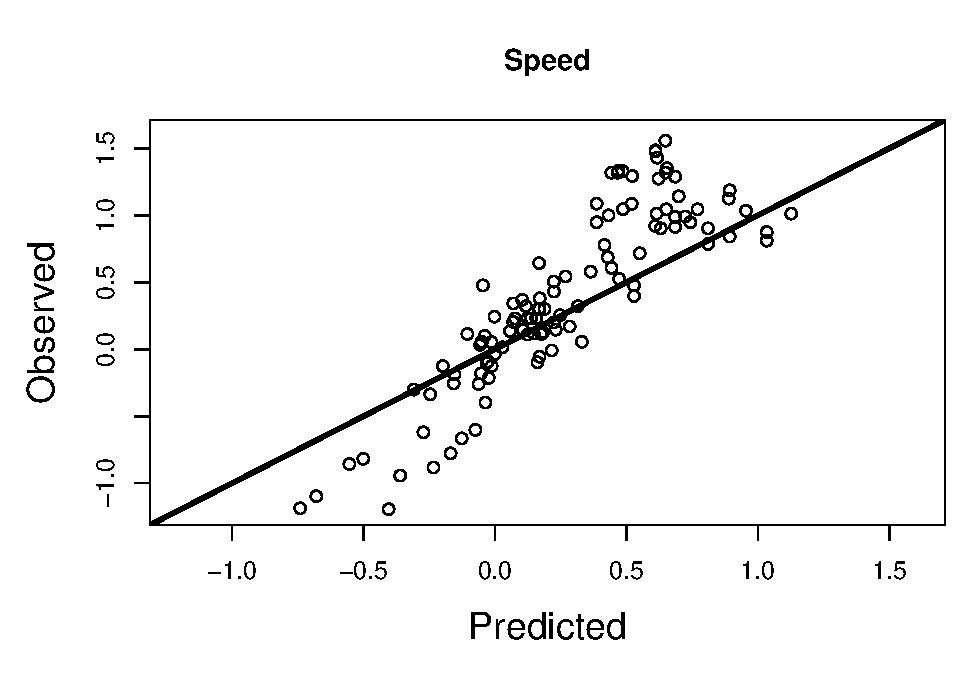
\includegraphics{Model_Fit_files/figure-latex/unnamed-chunk-7-1.pdf}
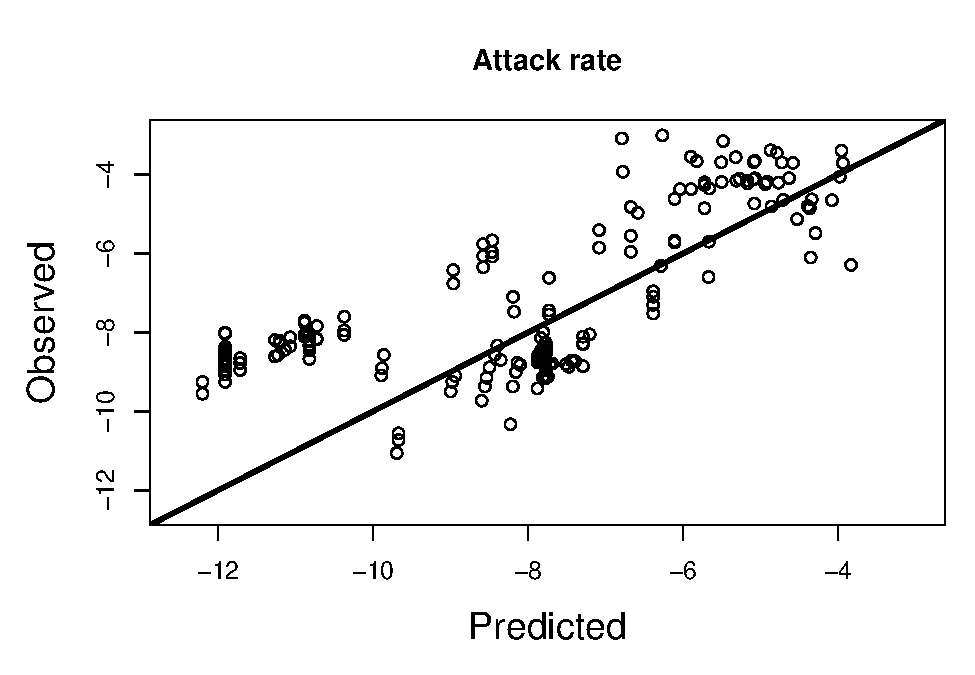
\includegraphics{Model_Fit_files/figure-latex/unnamed-chunk-7-2.pdf}
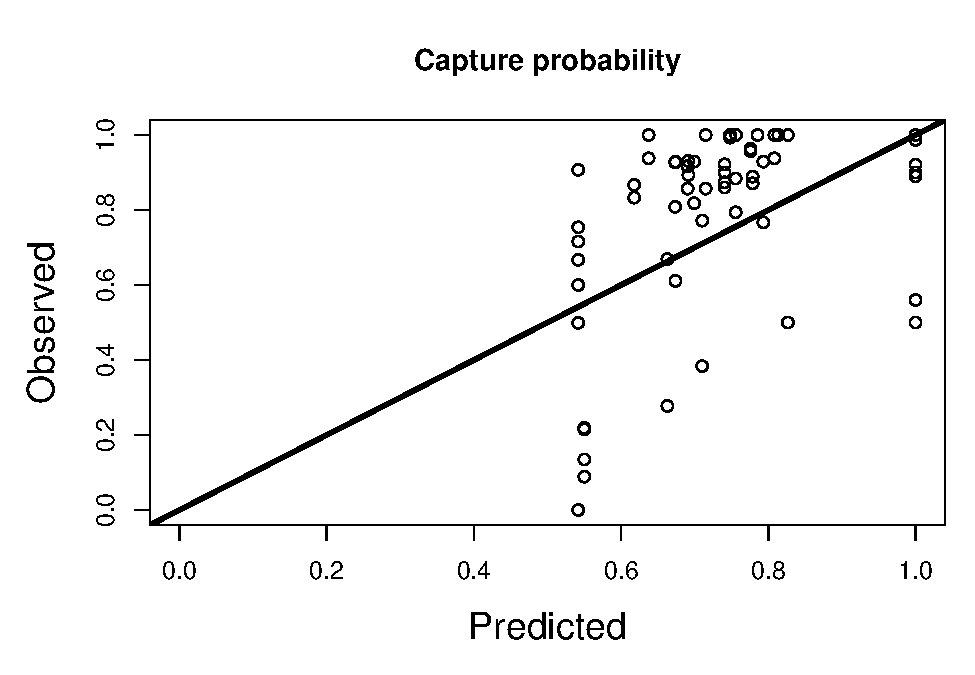
\includegraphics{Model_Fit_files/figure-latex/unnamed-chunk-7-3.pdf}
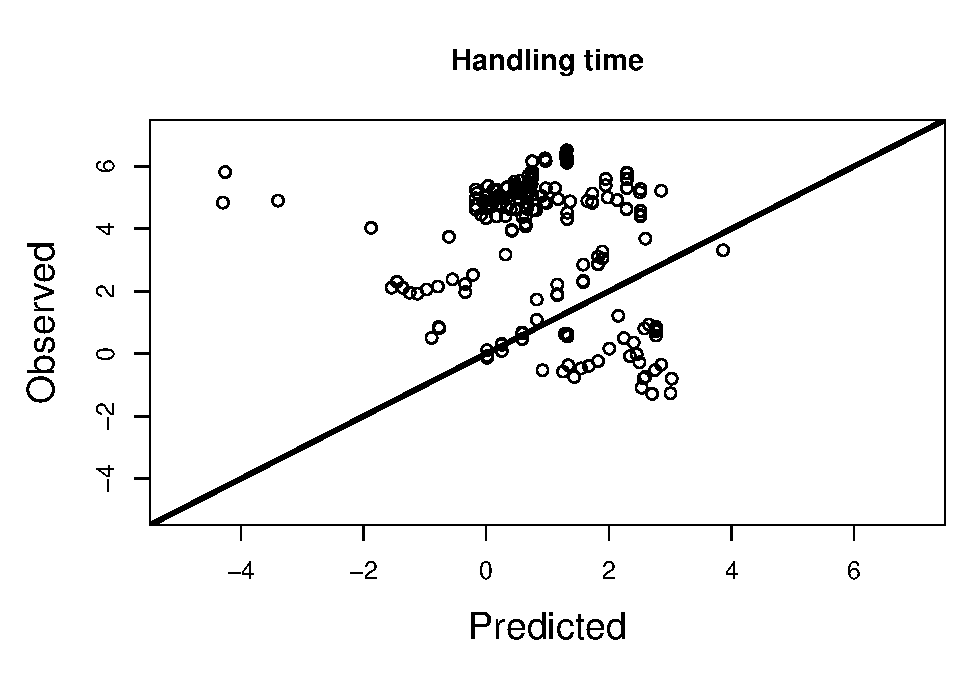
\includegraphics{Model_Fit_files/figure-latex/unnamed-chunk-7-4.pdf}
